\indent Acorde a lo solicitado, mostraremos distintos tipos de familias de casos para nuestro algoritmo, y adem\'as, daremos el tiempo estimado 
seg\'un la complejidad del algoritmo calculada anteriormente.\\

Luego de realizar varios chequeos de nuestro algoritmo, se pudieron elaborar una serie de casos puntuales:

\begin{itemize}
\item Hay m\'as canibales que arqueologos, es decir, no hay soluci\'on.
\item No hay canibales
\item Todos los canibales y arqueologos presentan velocidades iguales
\item Todos los canibales y arqueologos presentan velocidades distintas
\item Hay m\'as arqueologos que canibales con velocidades dispares
\end{itemize}

Dado estos estilos de familias y, como las combinaciones de arqueologos y canibales no se puede respetar en todos los casos desarrollamos un gr\'afico para cada familia con la funci\'on resultante de lo que demora nuestro algoritmo en obtener una soluci\'on posible para cada tipo de entrada dada.

\vspace*{0.3cm} \vspace*{0.3cm}
  \begin{center}
 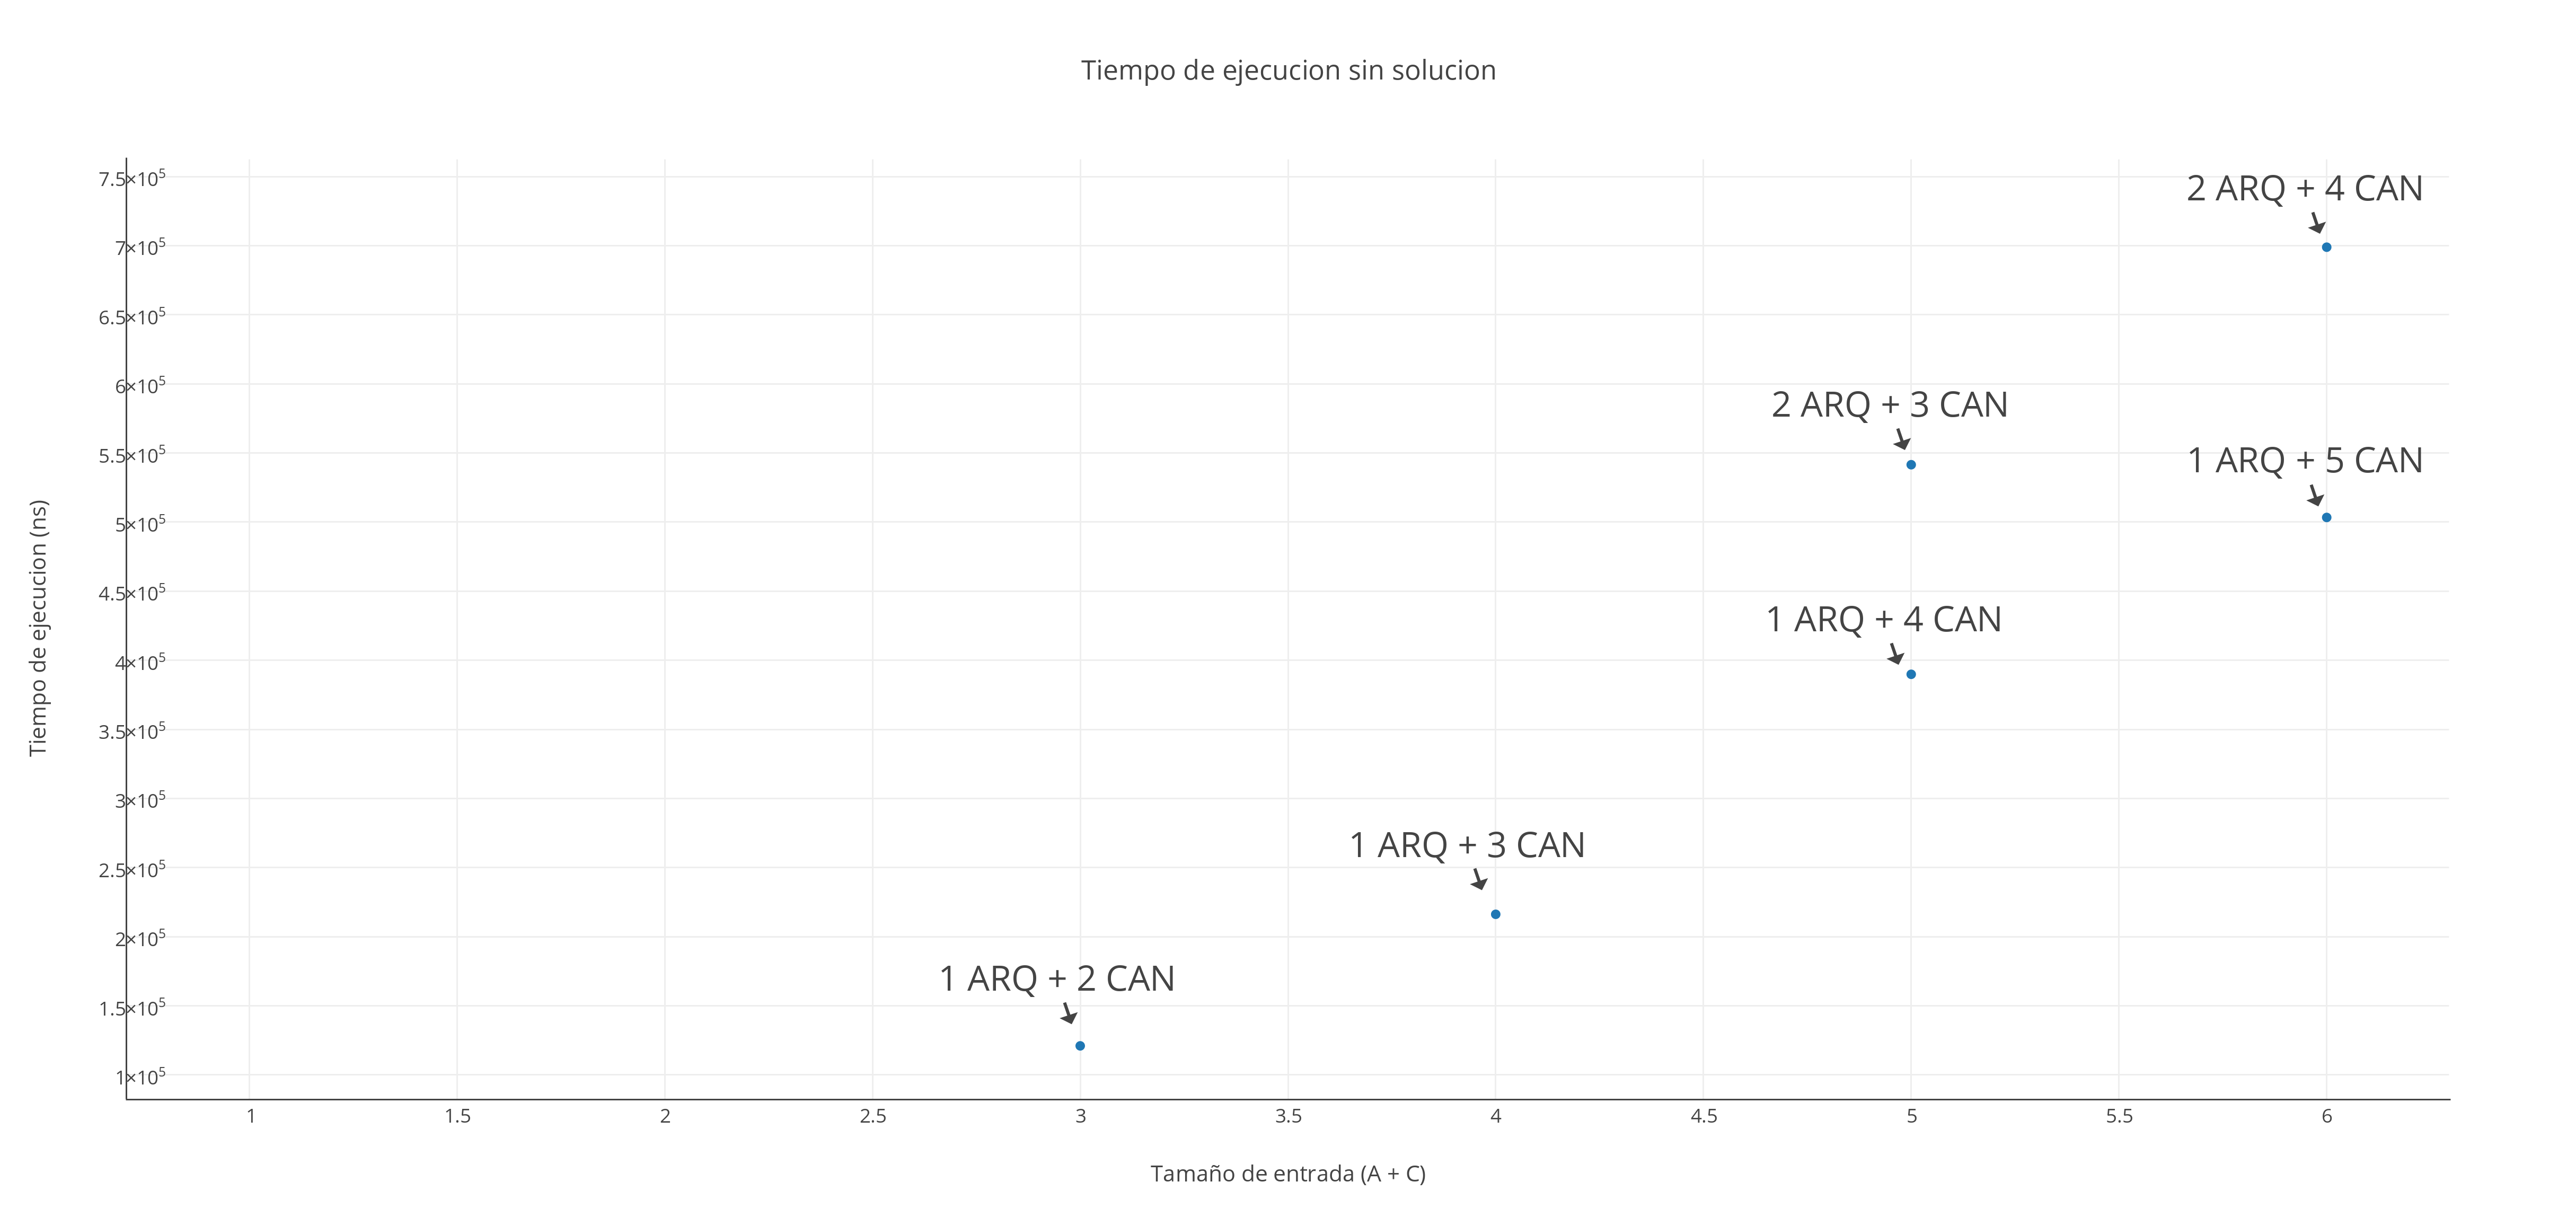
\includegraphics[scale=0.45]{./EJ1/sinsolucion.png}
 {$Gr$\'a$fico$ \ 1.1 - $Sin$ $Solucion$}
  \end{center}
  \vspace*{0.3cm}
 
 \vspace*{0.3cm} \vspace*{0.3cm}
  \begin{center}
 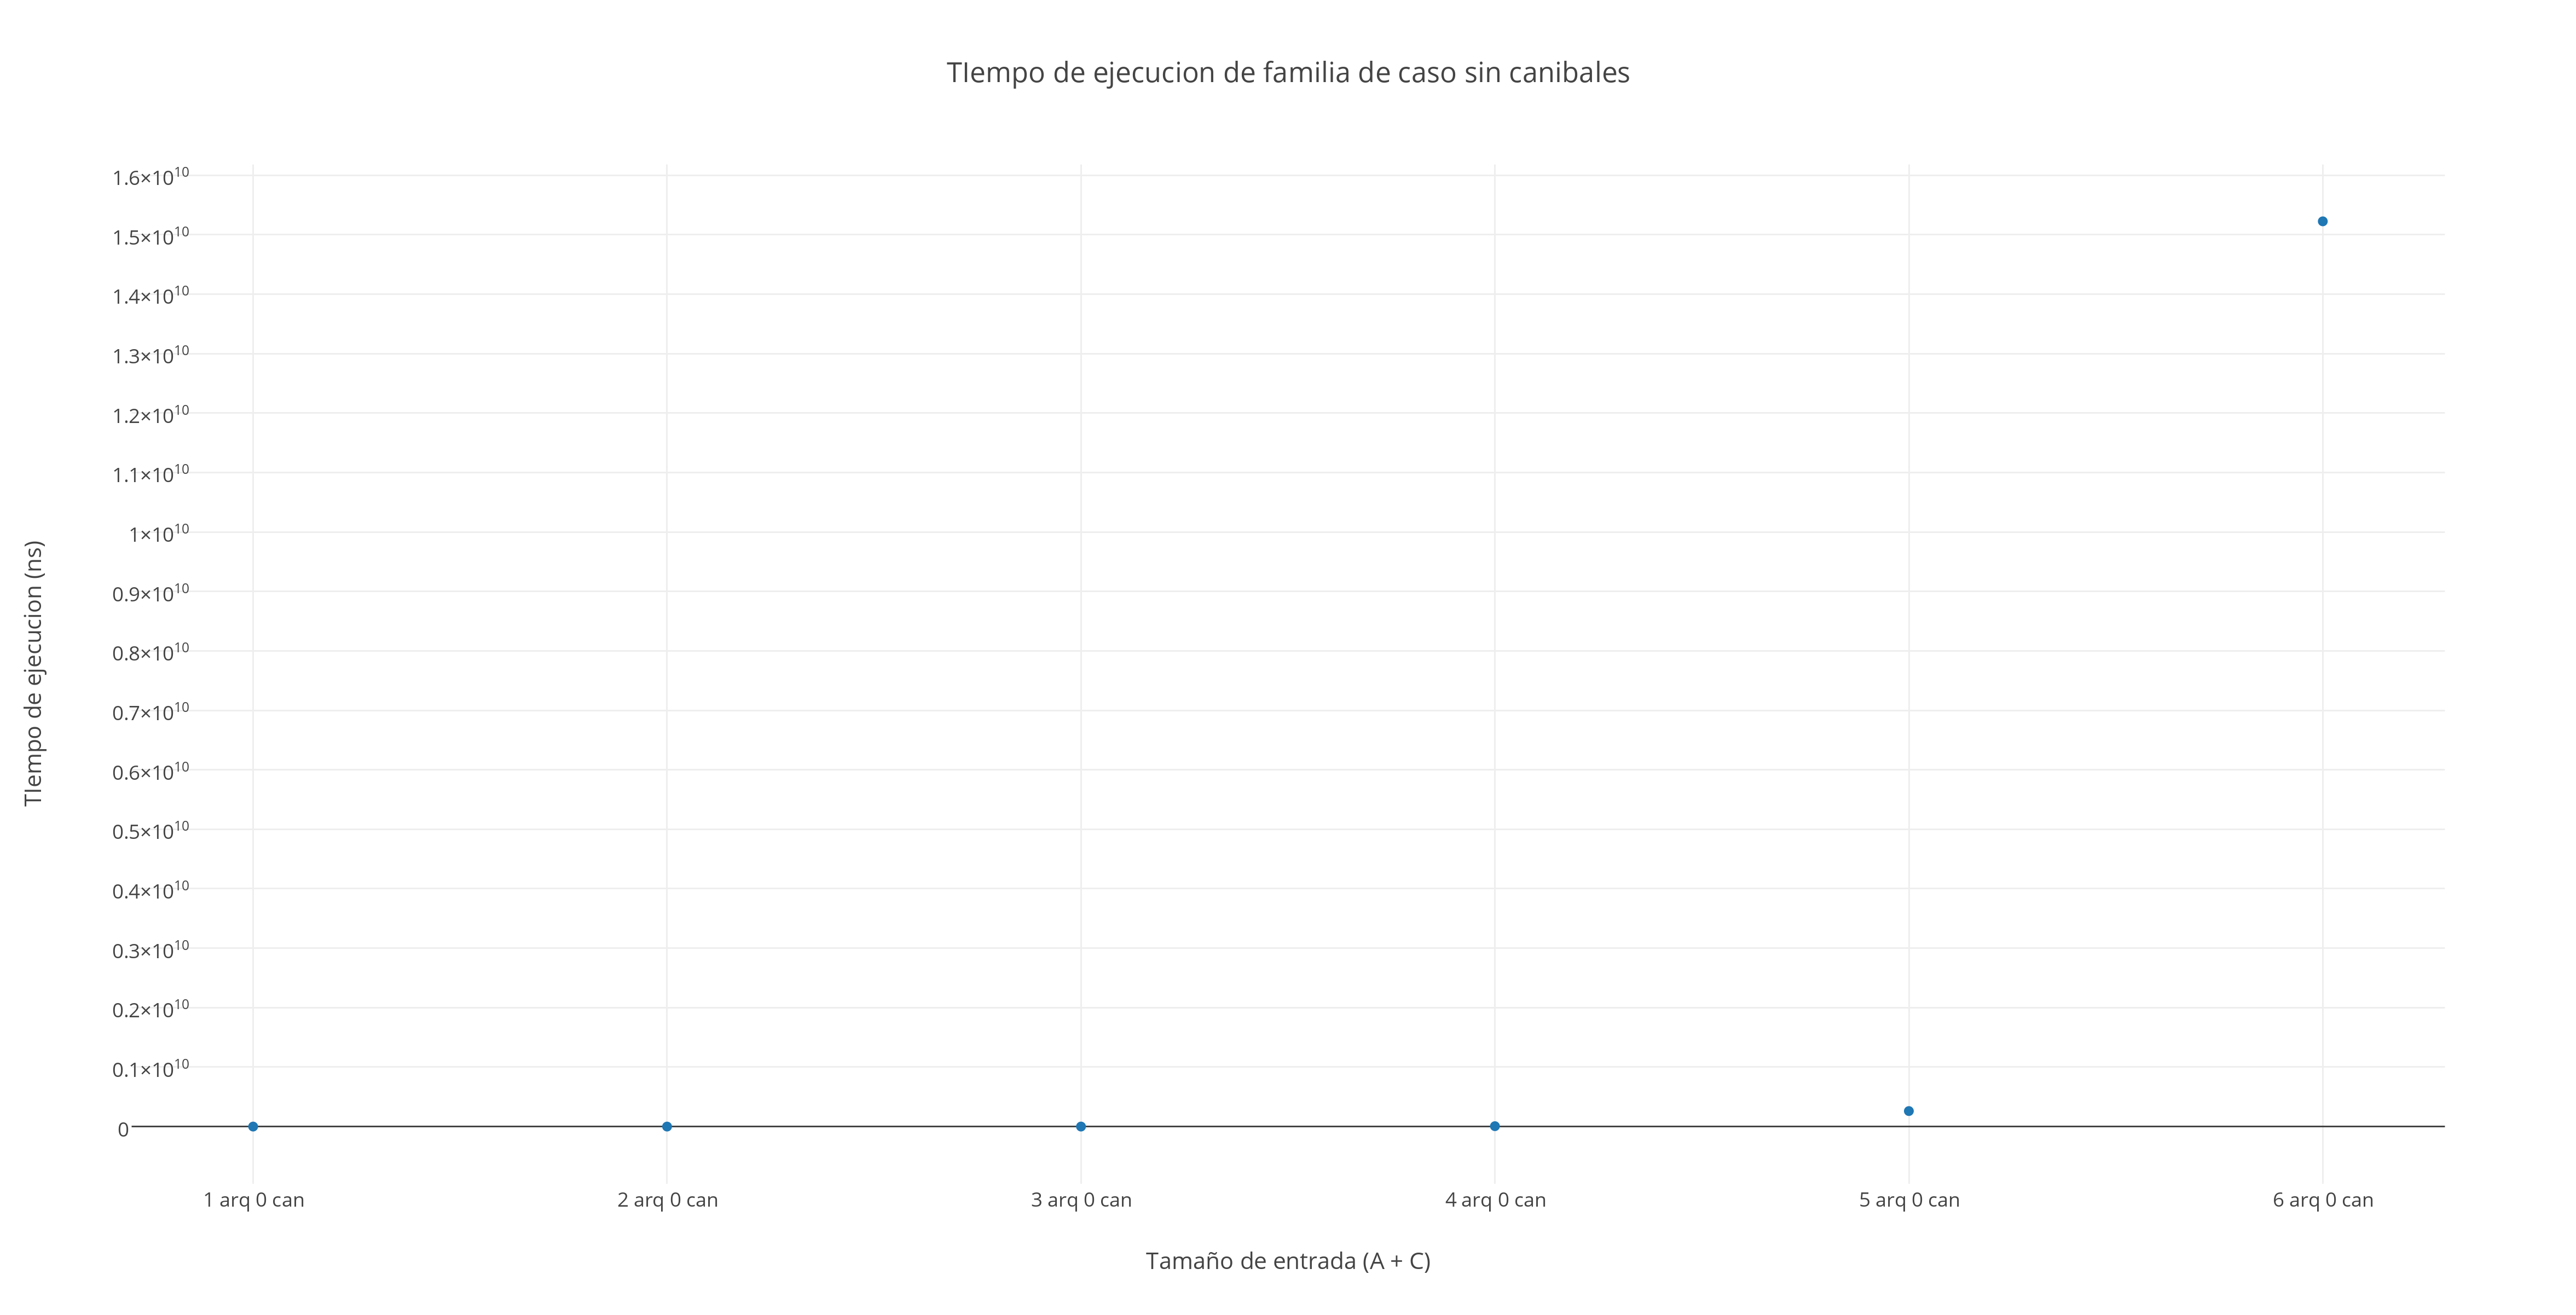
\includegraphics[scale=0.45]{./EJ1/sincanibales.png}
 {$Gr$\'a$fico$ \ 1.2 - $Sin$ $Canibales$}
  \end{center}
  \vspace*{0.3cm}
  
     \vspace*{0.3cm} \vspace*{0.3cm}
  \begin{center}
 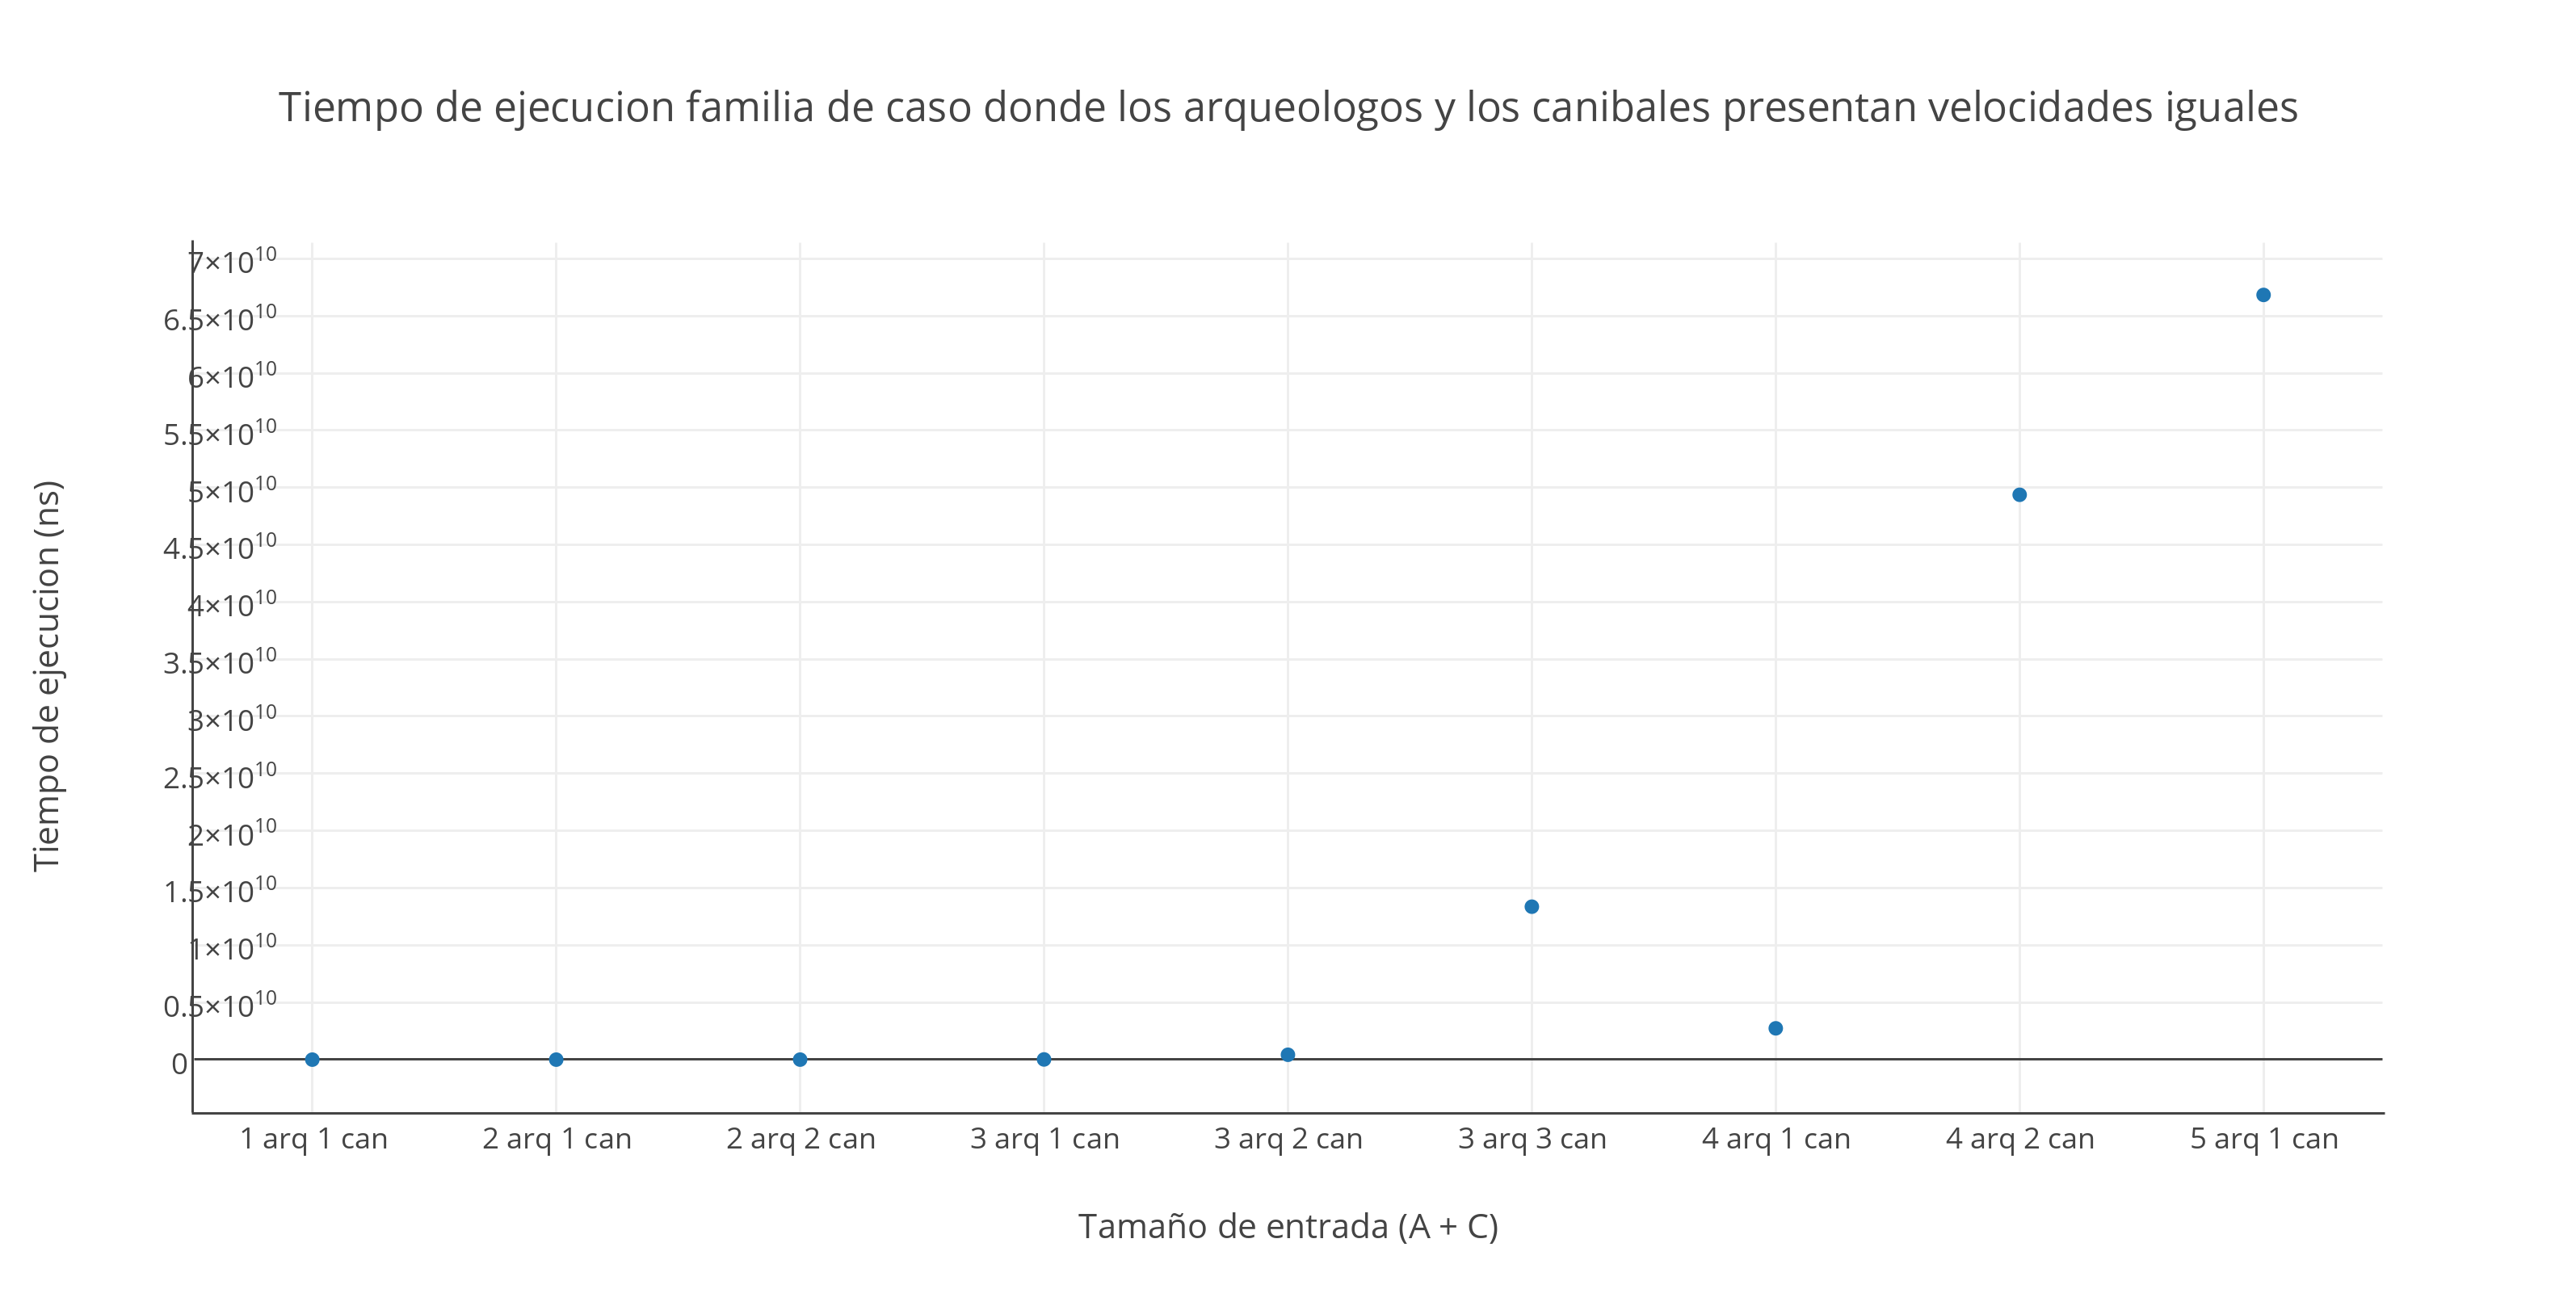
\includegraphics[scale=0.45]{./EJ1/velIgual.png}
 {$Gr$\'a$fico$ \ 1.3 - $Velocidades$ $Iguales$ $Para$ $Todos$}
  \end{center}
  \vspace*{0.3cm}
  
   \vspace*{0.3cm} \vspace*{0.3cm}
  \begin{center}
 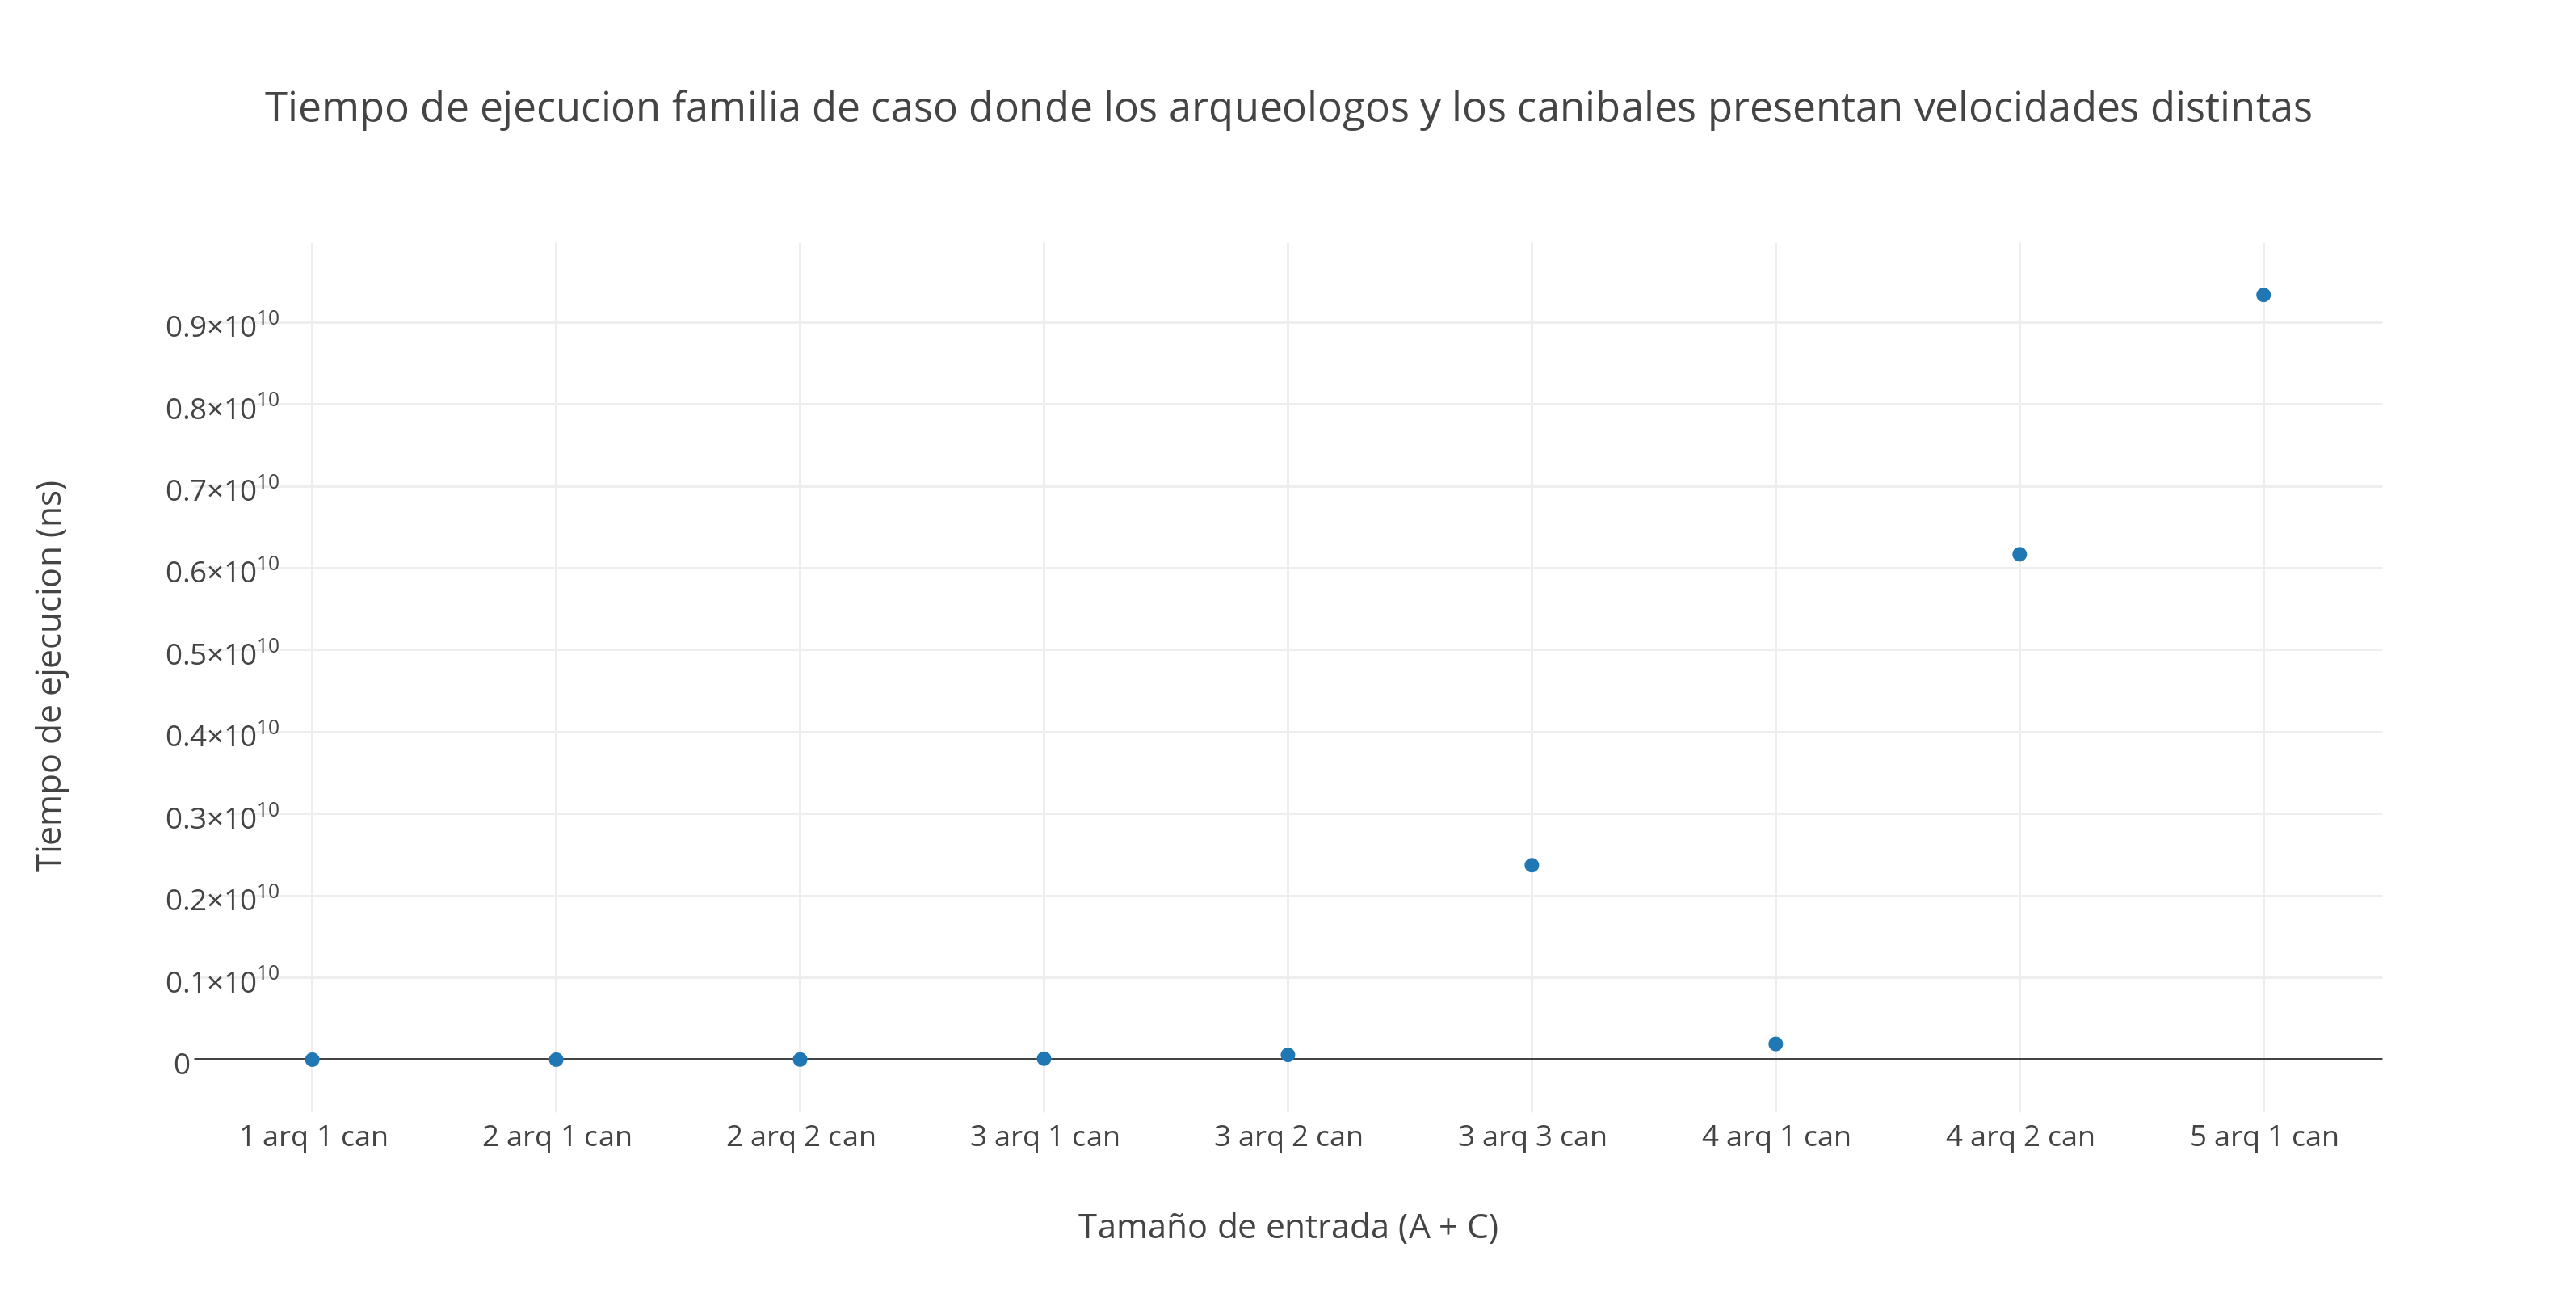
\includegraphics[scale=0.45]{./EJ1/velDistinta.png}
 {$Gr$\'a$fico$ \ 1.4 - $Velocidades$ $Distintas$ $Para$ $Todos$}
  \end{center}
  \vspace*{0.3cm}
  
  
   \vspace*{0.3cm} \vspace*{0.3cm}
  \begin{center}
 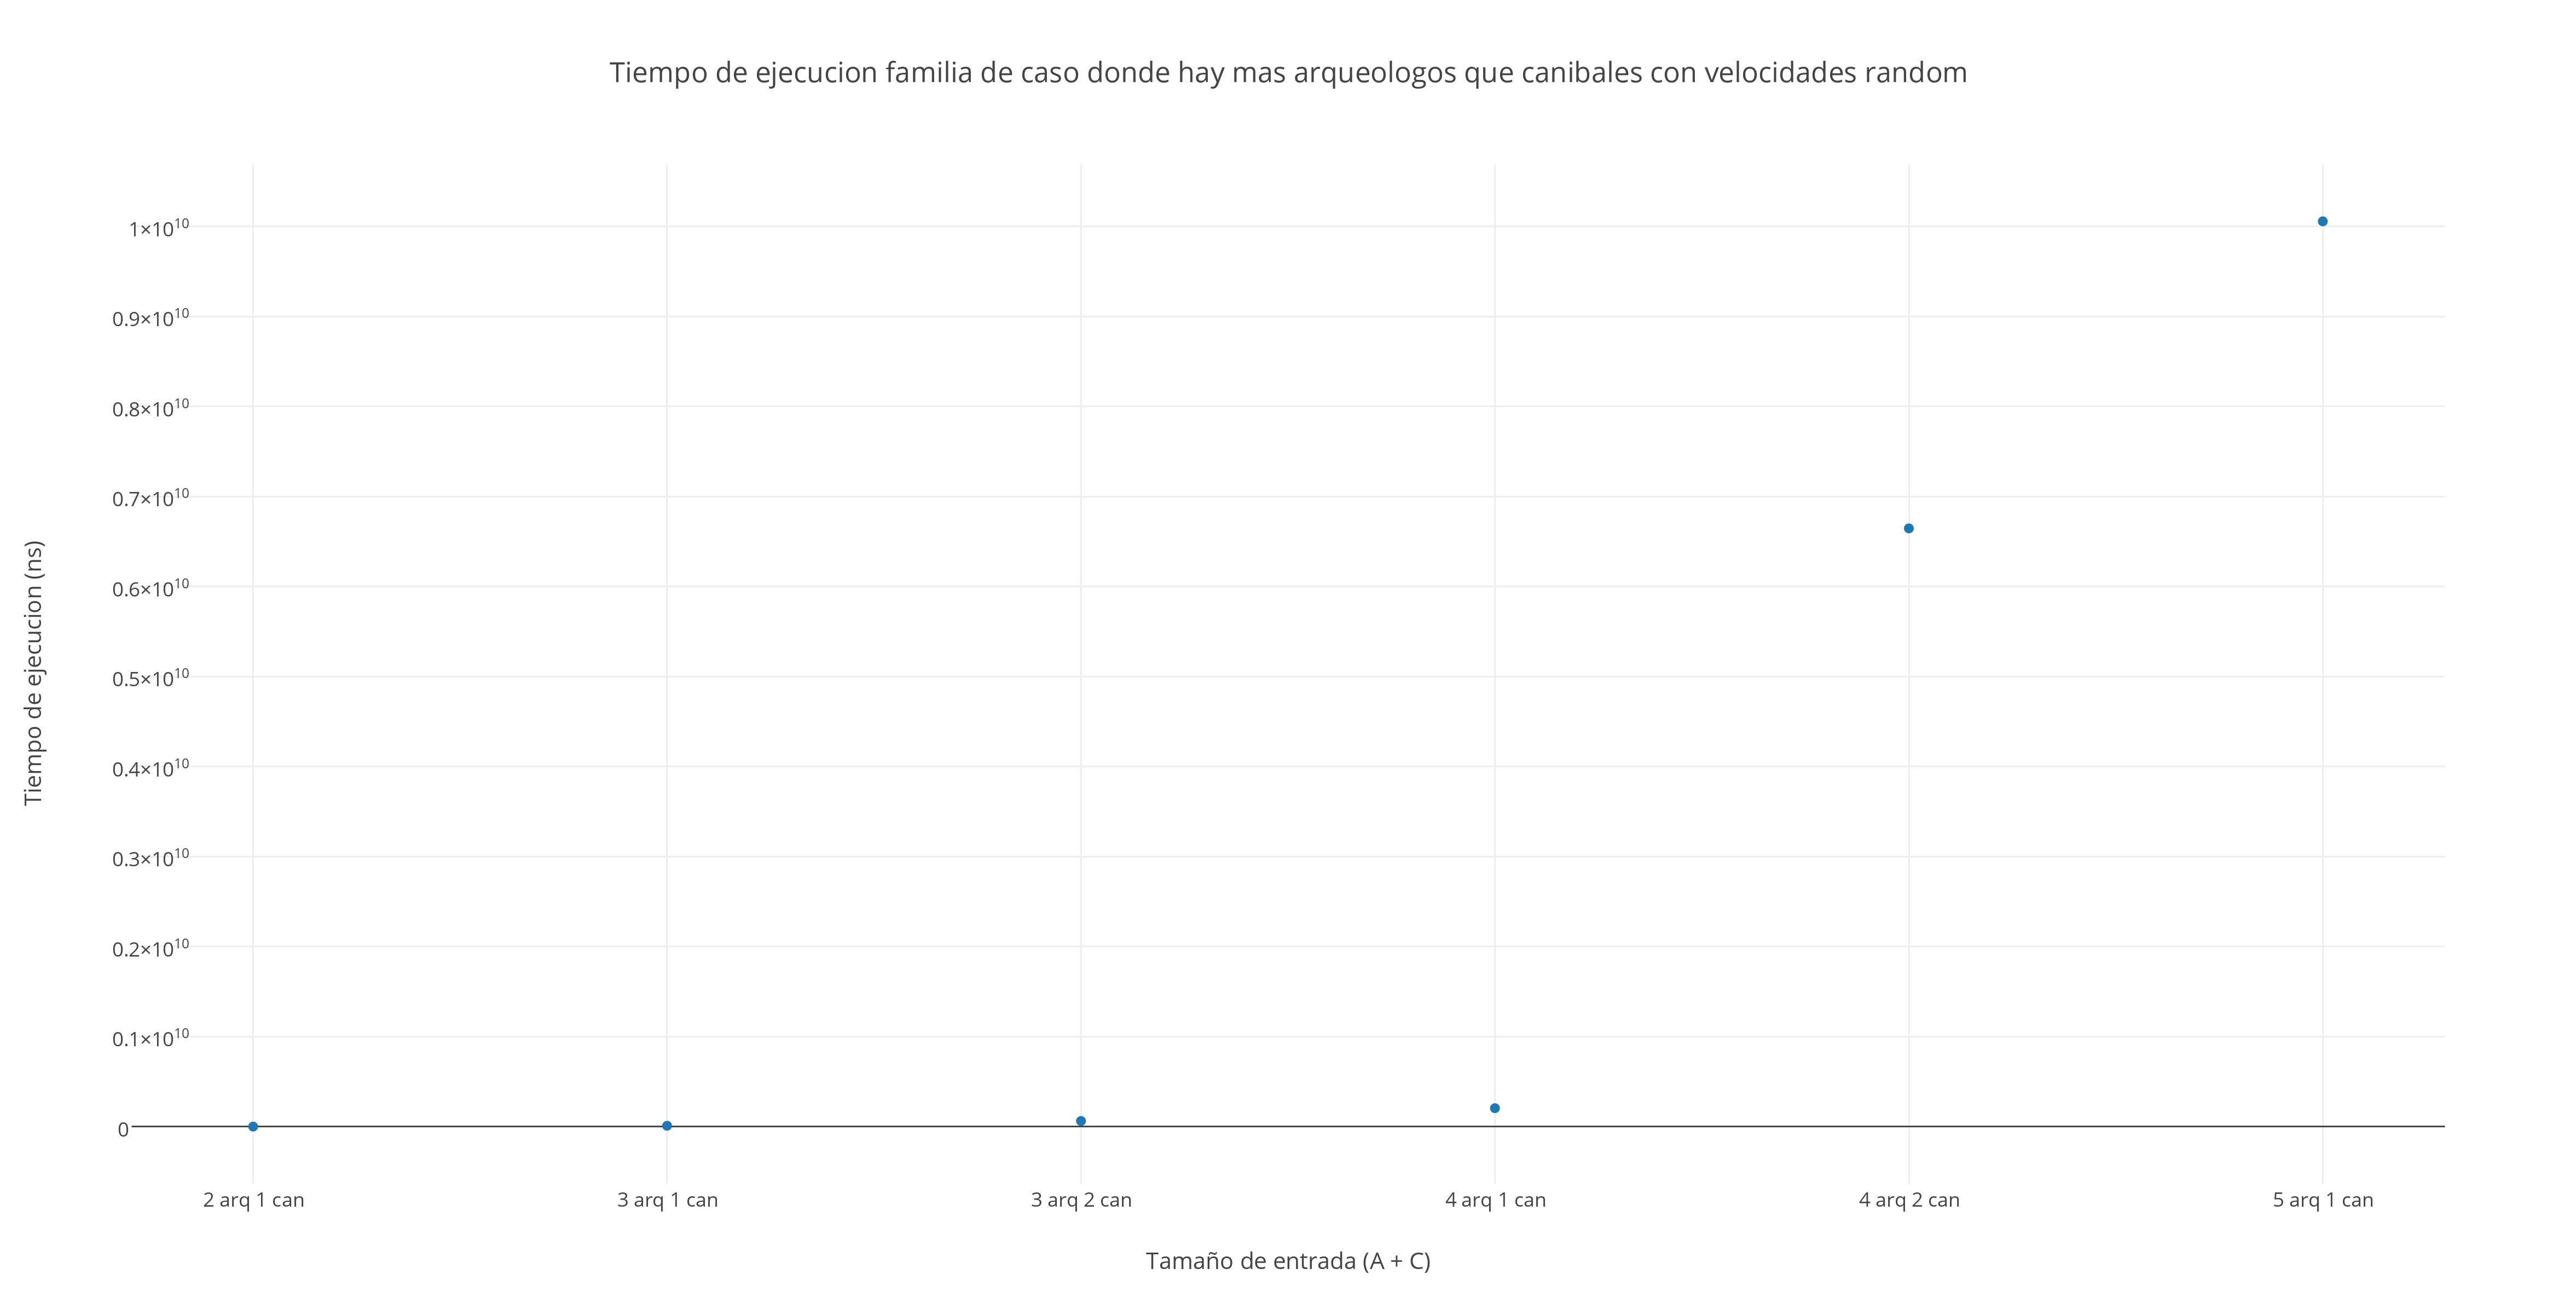
\includegraphics[scale=0.45]{./EJ1/velrandom.png}
 {$Gr$\'a$fico$ \ 1.5 - $Velocidades$ $Random$ $Para$ $Todos$}
  \end{center}
  \vspace*{0.3cm}
  
Luego de realizar dichas mediciones pudimos observar que todas las funciones representativas a cada caso son crecientes cuando el N (A + C) aumenta, exceptuando el caso sin soluci\'on (Ver gr\'afico 1.1) el cual tiene un m\'aximo con 2 arqueologos y 4 canibales y luego decrece, esto se da ya que cuando nuestro algoritmo va chequeando las ramas y cantidades de elementos verifica con mayor rapidez que hay m\'as cantidad de canibales que arqueologos cuando hay 5 canibales y 1 arqueologo que en el otro caso, esto se da ya que la diferencia entre canibal - arqueologo es mayor.
 Adem\'as, corroboramos que para los casos en los cuales no hay soluci\'on o no hay canibales se obtiene una mejor performance que para aquellos en los cuales hay soluci\'on siempre y/o hay canibales siempre como son los casos de velocidades distintas o iguales. \\
Es por esto que desarrollamos dos gr\'aficos comparativos para visualizar cual ser\'a nuestro mejor y peor caso.

En el primero trabajaremos con los que se obtiene una mejor performance. Cabe aclarar que debido a que las entradas para un caso no son compatibles en otros (por ejemplo, el caso sin soluci\'on contra el sin canibales), trabajamos con el valor de N final, el cual se obtiene de sumar la cantidad de arqueologos con la cantidad de canibales.\\

   \vspace*{0.3cm} \vspace*{0.3cm}
  \begin{center}
 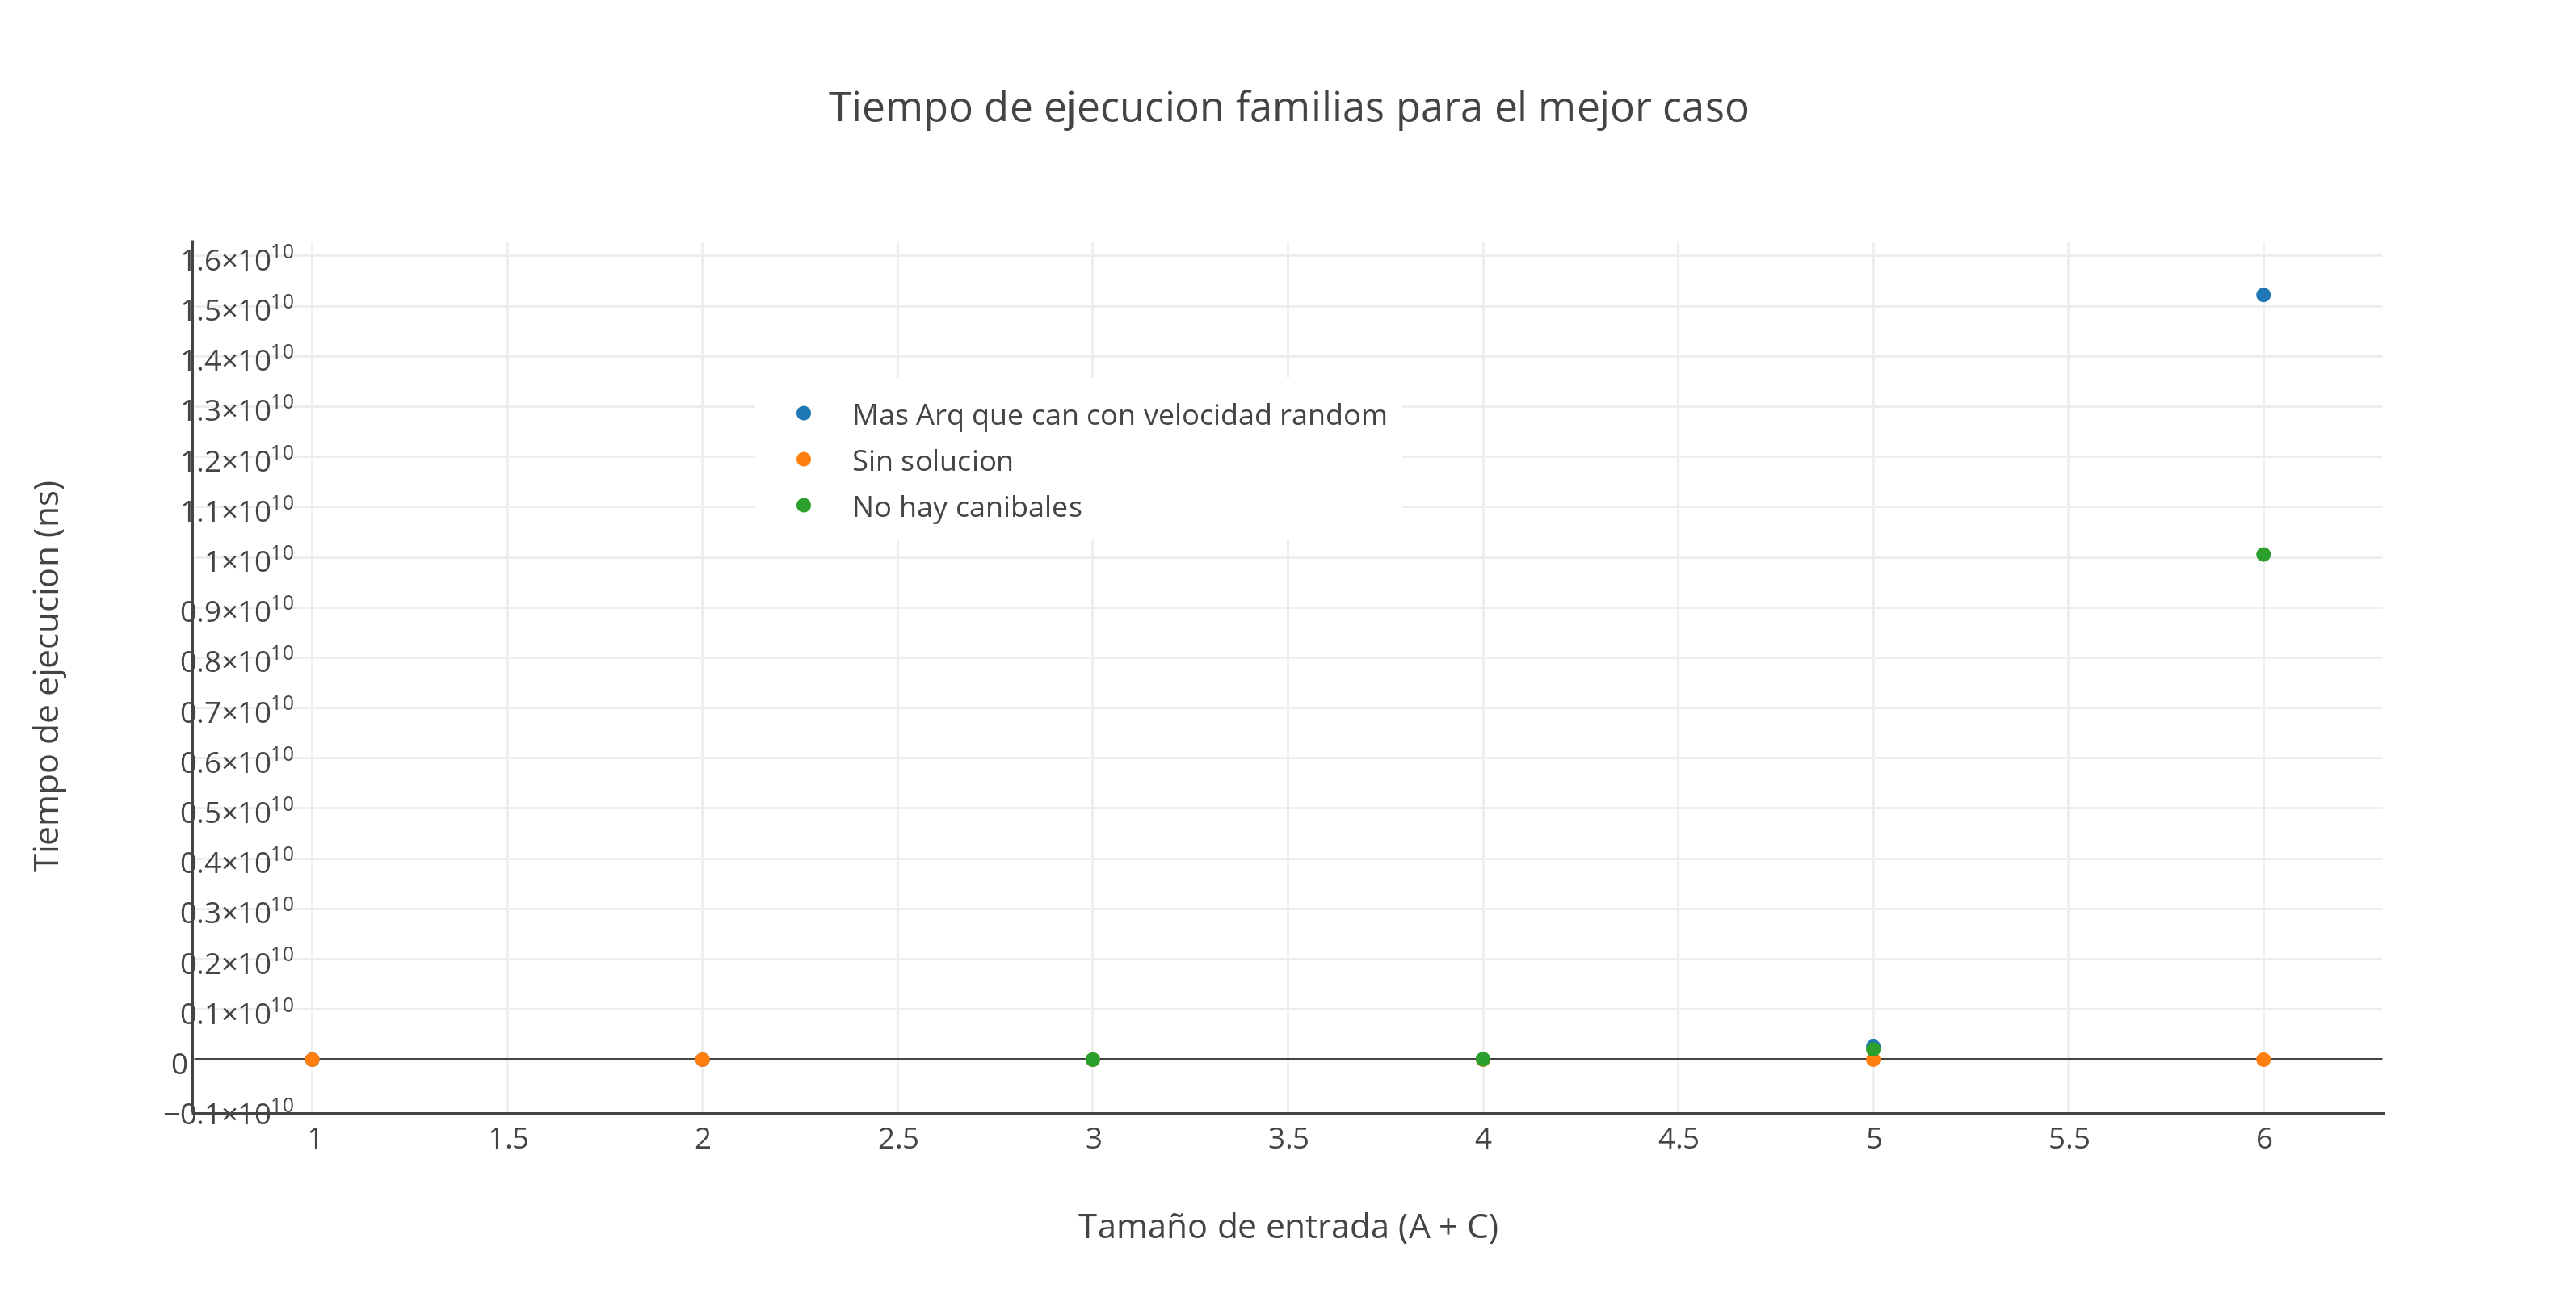
\includegraphics[scale=0.65]{./EJ1/comparativomejorcaso.png}
 {$Gr$\'a$fico$ \ 1.6 - $Comparativo$ $Mejor$ $Caso$}
  \end{center}
  \vspace*{0.3cm}

Se puede observar en el gr\'afico, tres funciones las cuales representan el tiempo de ejecuci\'on de las familias que resultan mas beneficiadas al trabajar con nuestro algoritmo:\\
\begin{itemize}
\item Hay m\'as canibales que arqueologos, es decir, no hay soluci\'on.
\item No hay canibales
\item Hay m\'as arqueologos que canibales con velocidades dispares
\end{itemize}

Como se observa en el gr\'afico la funci\'on representativa de la flia n\'umero 1, presenta una mejor performance en relaci\'on a las otras. Esto se debe a que nuestro algoritmo como  va chequeando y probando todos los posibles pares que viajen de un lado al otro, y, como inicialmente chequea que hay m\'as canibales que arqueologos imposibilitando un par posible, el algoritmo corta sin probar los posibles pares, finalizando su ejecuci\'on.

Luego de haber chequeado dichas instancias, pudimos llegar a la conclusi\'on que la familia de casos que presenta una mejor performance para nuestro algoritmo
es en el cual \textbf{Hay m\'as canibales que arqueologos, es decir, no hay soluci\'on}

Luego, para verificar el peor caso, desarrollamos otro gr\'afico de mediciones como enunciamos al principio el cual contendr\'a los peor casos posibles para nuestro algoritmo. Como dichos casos presentan las mismas entradas v\'alidas tanto en uno como en otro, fue posible graficarlos juntos mostrando el tiempo medido para cada entrada.\\

 \vspace*{0.3cm} \vspace*{0.3cm}
  \begin{center}
 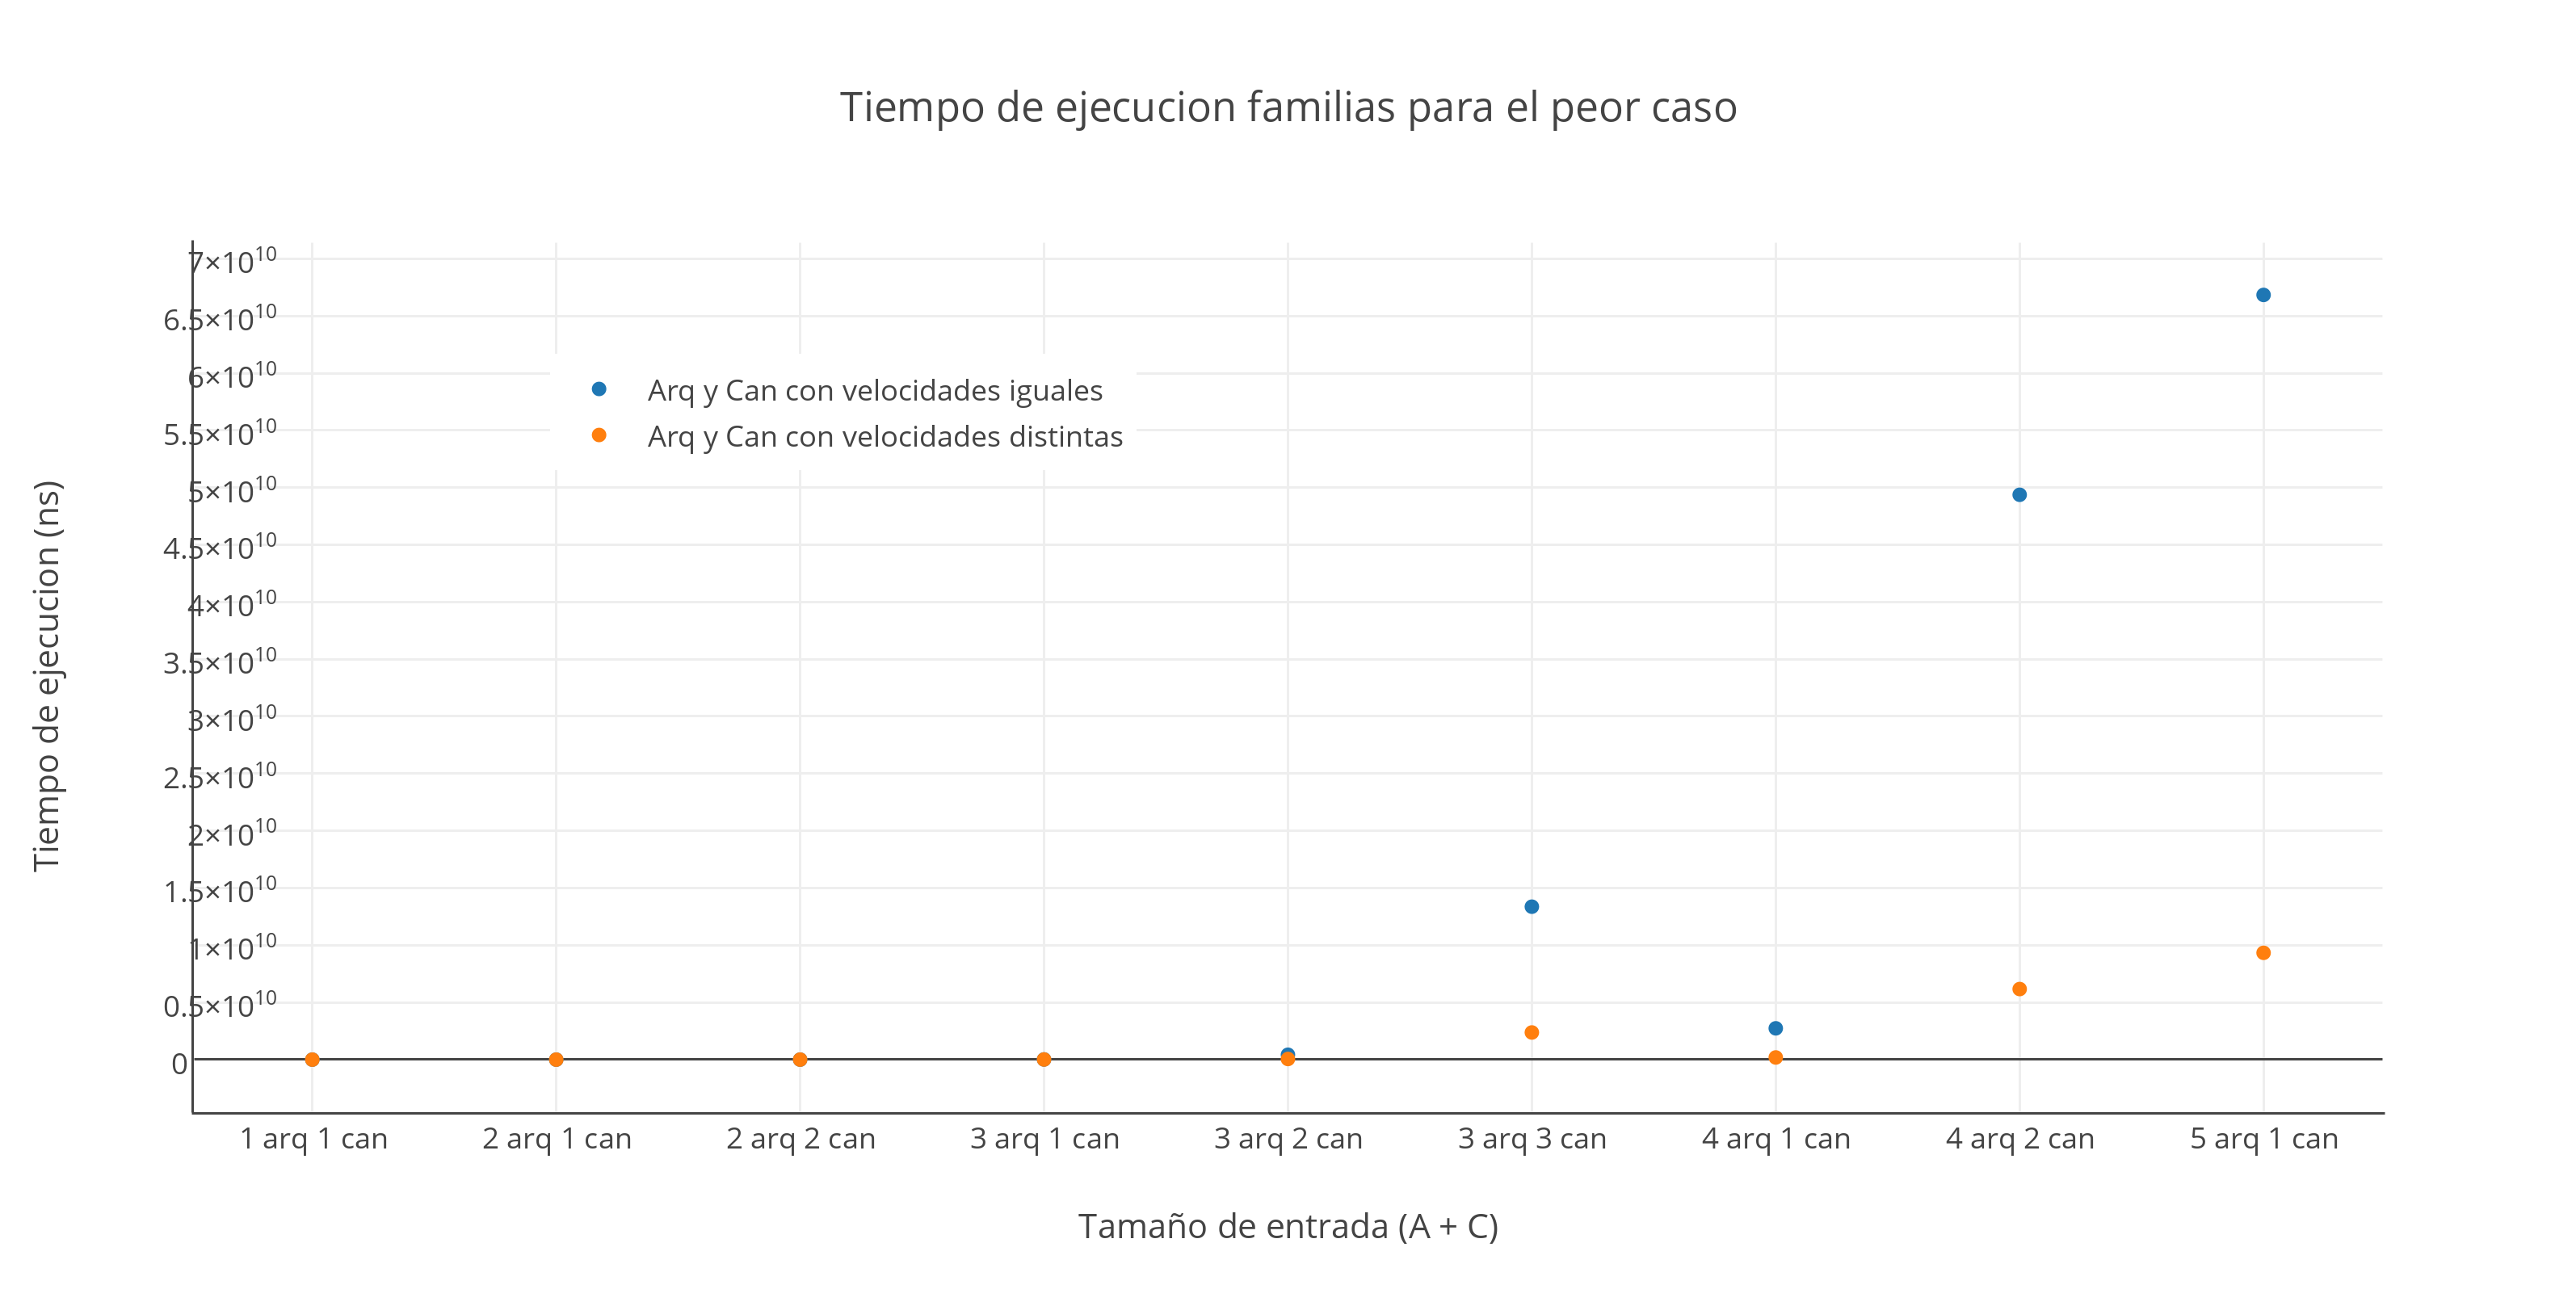
\includegraphics[scale=0.45]{./EJ1/comparativopeorcaso.png}
 {$Gr$\'a$fico$ \ 1.6 - $Comparativo$ $Peor$ $Caso$}
  \end{center}
  \vspace*{0.3cm}

Se puede observar en el gr\'afico, dos funciones las cuales representan el tiempo de ejecuci\'on de las familias que resultan menos beneficiadas a la hora de trabajar con nuestro algoritmo:\\
\begin{itemize}
\item Todos los canibales y arqueologos presentan velocidades iguales
\item Todos los canibales y arqueologos presentan velocidades distintas
\end{itemize}

Es posible observar en el gr\'afico que la funci\'on representativa de la flia n\'umero 1, presenta una peor performance en relaci\'on a la otra. Esto se debe a que nuestro algoritmo va chequeando y probando todos las permutaciones posibles de pares que viajen de un lado al otro, y, adem\'as como el mismo tiene realizado una poda la cual consiste en anular las ramas que tarden m\'as tiempo, dicha familia finalizar\'a m\'as tarde su ejecuci\'on en relaci\'on a la otra ya que al tener a todas las personas con las mismas velocidades dicha poda no podr\'a ser utilizada, generando de esta forma, el peor caso posible para nuestro algoritmo.\\

Por lo tanto, el peor caso para nuestro algoritmo ser\'a cuando \textbf{Todos los canibales y arqueologos presentan velocidades iguales, y dicha combinaci\'on de arqueologo - canibal tenga una soluci\'on posible}\\

Como se trabaja con pocos casos y la complejidad te\'orica es muy grande, como demostramos la misma es $O(N^{2^{N}})$, la misma no ser\'a posible graficar ya que el tiempo insumido por la misma es muy variante y al utilizar unicamente 6 elementos (teniendo en cuenta cualquier combinaci\'on de arqueologo y canibal, la suma de estos devuelve el mismo N) no es posible estabilizar dicha funci\'on y obtener datos consisos. Adem\'as, en caso de querer trabajar con elementos de mayor tamaño el tiempo insumido no es apto para los dispositivos f\'isicos en los que se los chequea.

